\chapter{Dataset}
\label{chapter:dataset}

In this chapter, we will provide information regarding the datasets that we used in our research. We will describe how we obtained a labeled dataset for training and also mention weaknesses that come with that dataset. We will take a look at the important properties of the logs. 
Also, we will pay attention to a couple of known anomaly scenarios that may occur in the system logs, and we will go through the dataset where they are captured. 
We use the anomalies for validation of our models. A validation dataset which contains anomaly free data will be described as well. 

All the datasets contain log traces gathered from multiple microservices comprising Motorola SmartConnect's Cloud Infrastructure Engineering development environments.
In order to obtain the logs, we came up with a pipeline (specifics of the pipeline are described in Chapter~\ref{data_collection}) that connects to the system, gathers and preprocesses them into such a form that the data can be fed to selected machine learning algorithms or plotted.
More on the preprocessing step can be found in Chapter \ref{methodology}.

\section{Datasets}
\label{dataset}
The data we feed to machine learning models make a great deal of difference. Therefore, we need to look at what data we are able to collect from the system in a both high level and also what are the properties of a single log entry.

The anomaly detection task can be reformulated as a classification problem with two classes: \textit{negative (anomaly)} class and \textit{positive (anomaly-free)} class. 

\textit{Negative} or \textit{normal} class is a category of a set of data, that is free of anomalies and represents expected (or normal) behaviour of a system that produces those logs. Negative data samples are labeled as $0$. \textit{Positive}, \textit{anomalous} or \textit{abnormal} class is the target class that we are interested in. It is assigned to log sequences which contain anomalies as $1$. The goal is to train the classifier to distinguish between positive and negative samples.

Motorola Solution's policy for storing historical data is that at every moment, we have at our disposal logs from before $30$ days until that moment. The stored interval can at times get even smaller if the amount of persisted logs exceeds a limit.

In Motorola, the development environment is further divided into two sub regions that we have access to. 
Let's call them \textit{experimental} and \textit{stable}. 

\textit{Stable} environment is in sync with master branches of the source code and is used for running exhaustive testing of the system every night. 

On the other hand, \textit{experimental} environment would be used by developers to deploy and examine side (feature) branches throughout their the day.

Due to confidentiality reasons, we do not have logs from \textit{production} environment at our disposal. It is one of the major setbacks, as the assumption would be that it contains different traffic. It can be also assumed that distribution of anomalies in the production dataset is different from both \textit{experimental} (more anomalies, some of them related to ad-hoc deployment not in \textit{production}) and \textit{stable}(less anomalies, less traffic). In general, the development environment produces vast amount of data, thousands of log messages per minute.

Next, we will provide a detailed description of characteristics of each of the datasets and how it was obtained. In Table \ref{table:datasets} is a summary of all datasets used in this thesis.

\subsection{Dataset Daily} 
This dataset reflects \textit{experimental} region of development environment. In such a setting it is natural (or even desired) for anomalies to occur.

We call the dataset of system logs produced by the region a \textit{Daily} dataset and we may also refer to it as \textit{mixed}, as it will contain both positive and negative data samples. 
The system is active during a working day when developers are testing new features. The amount of logs varies a lot depending on the tasks of the team. 
However, we are talking about tens of thousands of log messages per hour, even when the system is idle.

Unfortunately, such dataset in unlabeled, as it would require experts going through millions of lines of unstructured log messages to obtain them.

\subsection{Dataset Nightly}
At night, the system we are experimenting with undergoes tests in the \textit{stable} region. This phase of system's health check includes mimicking normal behavior of the telecommunication system. All the required set up of the infrastructure takes place and simulations of calls between groups of push-to-talk radios are happening. 
These tests are being re-run every night as a part of the nightly test suite. 
Usually, the test pipeline takes around 7 hours and produces roughly 2 millions of log messages.

In case the nightly tests are all passed, it should be sound that the collected data are either completely free of anomalies, respectively contain only a very small percentage of them. 
Therefore, we assume that the data collected during the nightly test phase, and it passes successfully, contains a vast majority of negative data samples and represents a normal, anomaly-free behaviour of the system. This statement strongly relies on the assumption that the functionality of the system is well covered by the tests (the relationship of our approach to anomaly detection and test code coverage is elaborated in detail in Section~\ref{code_coverage}). 

Hence, for our use case, we may also refer to \textit{negative} or \textit{normal} dataset as the \textit{Nightly} dataset interchangeably.

Therefore, the logs that are collected at night from a system like this should be suitable candidates for one-class classification algorithms, as well as generating a labeled dataset for testing purposes, which we will explain later in this chapter.

However, the data that the system under the nightly testing is producing, slightly differ from the live production environment. The main difference is that the scenarios the test suite generates are serialized, meaning that maximum one call is taking place at each moment. 

On the other hand, the live production environment is not limiting the number of broadcasts at a time. Therefore, the logs of the production environment may include much higher counts of some events.

Although this might be argued as a weakness of our nightly dataset, as we have described windowing operation of our preprocessing phase in Chapter \ref{methodology}, we will always consider a sequence of logs and the counts of event types in that log sequence in a fixed time window. Therefore, even if the data will look different in terms of individual log entries, we believe the final feature representation passed to the ML algorithm should be very similar.

As it is incredibly challenging to obtain labels in log data, we have decided to use the Nightly data, despite it's possible drawbacks and slightly artificial character.

The Nightly contains logs from the night of January 24, 2021.

\subsection{Dataset Nightly Test}
This dataset is collected the same way as the Nightly and should satisfy all the properties, however it has been recorded on a different day. Therefore the timing is different and the tests are benchmarking different version of source code of the SmartConnect system.

We use this Nightly Test mainly to show that similar distribution of arbitrary dataset gathered from nightly testing can be assumed.

Nightly Check contains logs from the night of January 22, 2021.

\subsection{Dataset Anomalies}

This dataset contains versions of both of the anomaly scenarios described later in Section~\ref{anomaly_types}. 
The anomalies were achieved by killing Kubernetes Pods responsible for correct operation of a specific type of service. 
At the same time, users were trying to establish, or were in a call.

This dataset records in total 23 instances of anomaly scenarios and was created by merging logs from two days - 25th and 28th of January, 2021.

\subsection{Dataset Glostrup Calling}

On the contrary, dataset Glostrup Calling is comprised of anomaly free calls between Motorola Solutions two-way radios. 
The \textit{experimental} environment was set in such way that nothing else was interfering with the calls. Therefore the resulting logs can be considered \textit{normal} data.

The trace records multiple calls that were carried out during 8 minutes on 3. February 2021.

\section{Dataset Test with Labels} 
\label{section:testset}
Unsupervised learning does not require data to be labeled to detect anomalies, as it assumes that the majority of data points are normal. This is very beneficial in our situation, where obtaining labeled data is extremely difficult. However, an absence of labels represents a difficulty when it comes to model evaluation phase.

Unlike a supervised learning, where one can compare predictions directly with the actual labels to assess the quality of the machine learning model, in unsupervised learning, there is no way to do that.

In our thesis, the majority of data are unlabeled data. In order to validate the proposed approaches, we had to develop the testing dataset ourselves.

To get a better idea what kind of data comprises a manually generated testing dataset, we provide a pie chart of test set composition in Figure \ref{fig:testset-composition}. It is important to note here that the number $131$ represent the amount of extracted log sequence, therefore the number of underlying log message samples is much higher.

Getting the negative class representation is trivial. As we mentioned earlier in this chapter, we consider Nightly data obtained from the testing phase as normal data samples. To create the normal part of the dataset, we gather another set of data from the testing, that were previously unseen in the training phase. 

On the other hand, the positive samples need to be manually labeled. To avoid error while assigning labels, we introduce some known anomaly scenarios, which are expected to occur in our real-life dataset. These scenarios can be reproduced, we can gather the data and label them as anomalies. 

This is not an ideal testing dataset, but not all anomalies are known and can be obtained. It provides a reasonable tool to measure how well our models are doing. We will also test the models on solely normal data to detect false positives. 

\begin{figure}[h]
    \centering
    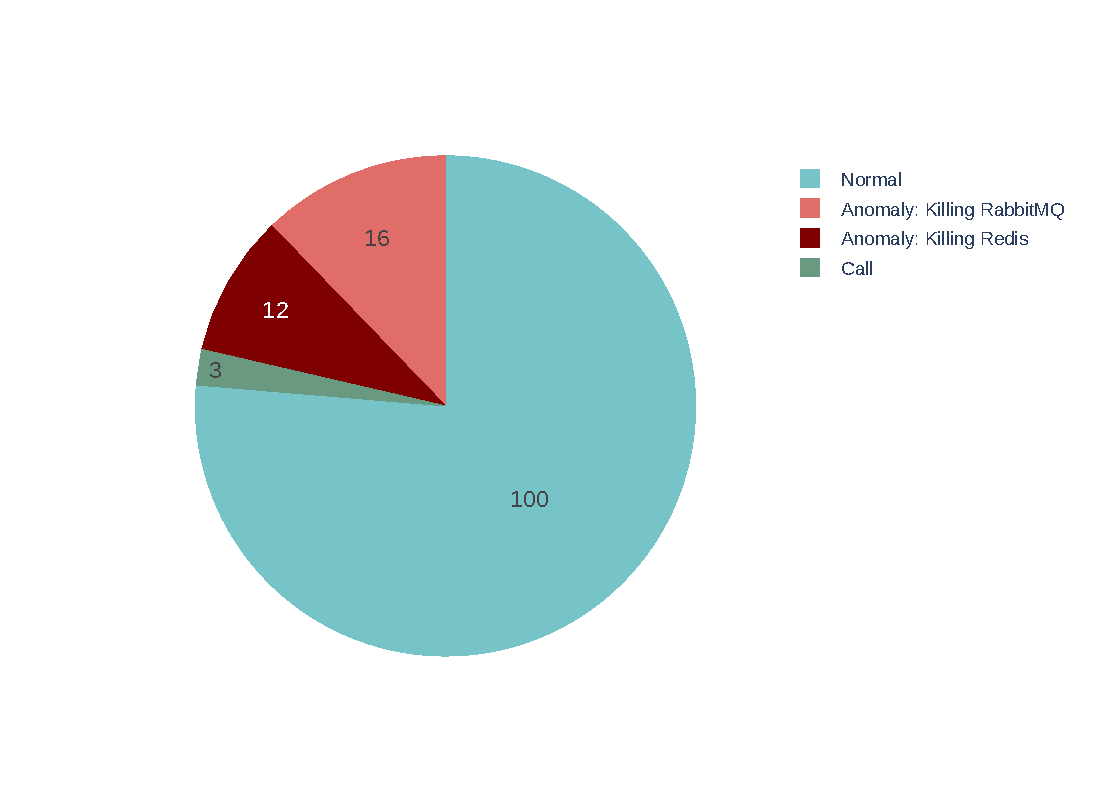
\includegraphics[width=0.8\textwidth]{img/testset-composition.pdf}
    \caption{Testing dataset composition. A manually collected and labeled dataset is composed of 131 log sequences, with each log sequence gathered within two minute window. The value on each section of the pie chart gives the number of log sequences of a respective type of log messages it contains. Normal and Call sections of the pie chart both represent normal, anomaly-free behaviour, whereas Killing RabbitMQ and Killing Redis are anomalies. }
    \label{fig:testset-composition}
\end{figure}

\begin{table}[!h]
\centering
\resizebox{\textwidth}{!}{\begin{tabular}{@{}lcr@{}}
\toprule
\textbf{Dataset Name} & \textbf{Log Entries}       & \textbf{Size}  &\textbf{Time Span}  \\ \toprule
\textcolor{customDarkBlue}{\textbf{Daily}}           & $539\,372$    & $2.84$ GB     & \footnotesize{ 26/1/2021 6:00  -  26/1/2021 21:00 }     \\ \midrule
\textcolor{customDarkBlue}{\textbf{Nightly}}         & $1\,362\,004$ & $4.24$ GB     &  \footnotesize{24/1/2021 21:00  -  25/1/2021 3:50}      \\ \midrule
\textcolor{customDarkBlue}{\textbf{Nightly Test}}    & $1\,373\,919$ & $4.47$ GB     &  \footnotesize{22/1/2021 21:00  -  23/1/2021 3:43}      \\ \midrule
\textcolor{customDarkBlue}{\textbf{Anomalies}}       & $805\,614$    & $3.6$ GB      & \footnotesize{ 25/1/2021 15:40  -  25/1/2021 17:00,  28/1/2021 15:25  -  28/1/2021 16:00}    \\ \midrule
\textcolor{customDarkBlue}{\textbf{Glostrup Calling}}    & $1904$    & $15.82$ MB    &  \footnotesize{3/2/2021 9:40  -  3/2/2021 9:47} \\
\bottomrule
\end{tabular}}
\caption{Summary of all the log datasets we worked with in our research on anomaly detection.}
\label{table:datasets}
\end{table}

\section{Log Properties}
The services record 33 properties per single log entry. Out of the 33 log properties, we decided to look only at \texttt{msg} and \texttt{timestamp} as the others (such as kubernetes pod name, process id of the service generating the log, etc. full list of the individual log properties are attached in Appendix~\ref{appendix:log-properties}) or are too specific, such as \texttt{pod}.
Including fewer predictor variables should in general avoid us overfitting, make the final model more transparent and easier to troubleshoot.
Therefore, in order to produce as general solution as possible, we stick only to those two predictors.

\subsection{Format of Log Properties}
Messages are strings and we assume they follow the logic that we described in Section~\ref{log_template_mining} on log template mining. In other words, we expect that they are generated by code in such a way, that we can think of them as a product of constant and variable parts. Consequently, log messages can be further categorized using event types.

Timestamps are in the format of \texttt{YYYY-MM-DD'T'HH:mm:SS.sss'Z'}. The format string specifies that year (YYYY) is a four digit zero padded number, month (\texttt{MM}), day (\texttt{DD}), hour (\texttt{HH}), minutes (\texttt{mm}) and seconds (\texttt{SS}) are two digit zero padded numbers and milliseconds(\texttt{ssss}) is a three digit zero padded number. The time part is separated from date by a single \texttt{T} character and the whole timestamp ends with a letter \texttt{Z}.

\section{Types of Anomalies}
\label{anomaly_types}
In this section, we present a couple of known anomalies that we will trace in order to test our solution.
We are going to benchmark our approaches and models against these known anomalies that can be easily simulated and can reproducible. 
However, the objective is to be also able to detect anomalies that we do not have a prior knowledge of.
In other words, we aim to identify even anomalous scenarios that are spotted for the first time in the production environment and do not appear in our training and testing dataset.

\subsection{Cache Outage}
In this anomaly, a cache storage that is orchestrating the call logic is taken down and radios that are in a call at that moment bonk as they are unable to communicate with each other.
In response to that, the storage service recovers itself automatically, usually in no more than 2 seconds. After that, broadcast should continue.

As mentioned in Section~\ref{architecture:caching} on caching in Motorola SmartConnect, Redis is used for caching, therefore we may also refer to this anomaly as \textit{Killing Redis} or similar.


\subsection{Message Broker Out of Service}
Similarly, an important entity in the SmartConnect microservices system is the message broker that allows for communication across services. In this scenario, all the brokers are killed, therefore the network of microservices is broken and messages cannot be passed until the brokers recover.

Again, in Section~\ref{architecture:messaging} we discuss how messages are passed in SmartConnect's microservices architecture. RabbitMQ is the specific message broker deployed, so we may refer to this anomaly as \textit{Killing RabbitMQ} in the text.

% https://pure.tue.nl/ws/portalfiles/portal/142685995/sci_2019_Lomagin_Egor.pdf